\documentclass{beamer}
\usepackage[english,russian]{babel}
\usepackage[utf8]{inputenc}
\usepackage{amsmath}
\usepackage{hyperref}
\usetheme{Warsaw}
\usepackage{listings}
\usepackage{xcolor}
\usepackage{tikz}
\usetikzlibrary{graphs}
\usepackage{algpseudocode}

\lstset{
    frame=tb,
    tabsize=4,
    showstringspaces=false,
    numbers=left,
    commentstyle=\color{green},
    keywordstyle=\color{blue},
    stringstyle=\color{red},
    emph={baz},
    emphstyle=\textbf
}
\begin{document}

\title{SAT/SMT solvers\ \newline 11. Symbolic execution}
\author{Roman Kholin}
\institute{Lomonosov Moscow State University}
\date{Moscow, 2023}

\begin{frame}
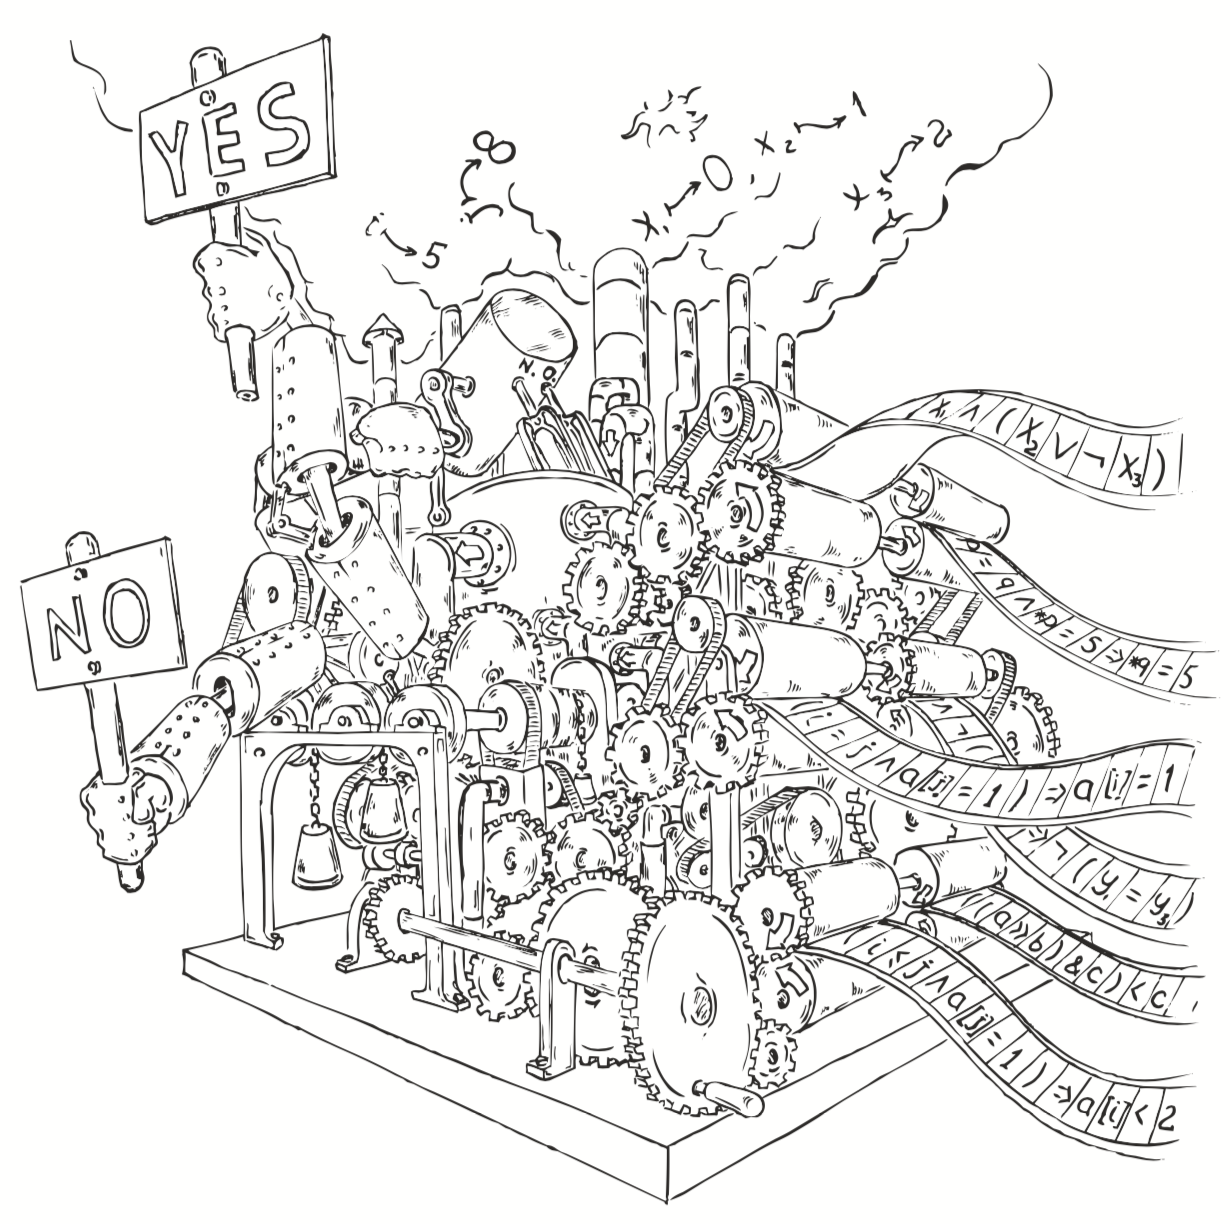
\includegraphics[scale=0.5]{../decision-procedure.png}
\end{frame}

\frame{\titlepage}

\begin{frame}{Whe could used}
\begin{itemize}
\item Dynamic analysis
\item Program correctness
\item Test generations
\item Taint analysis
\end{itemize}
\end{frame}

\begin{frame}[fragile]{Concrete execution}
\begin{minipage}{0.49\textwidth}
\begin{lstlisting}[language=C++]
void foo(int x, int y) {
    int t = 0;
    if (x > y) {
        t = x;
    } else {
        t = y;
    }
    if (t < x) {
        assert false;
    }
}
\end{lstlisting}
\end{minipage}
\hfill
\begin{minipage}{0.49\textwidth}
\begin{center}
\begin{tabular}{ | l | l | l | }
\hline
$X$ & $Y$ & $T$ \\
\hline
4 & 4 & 0 \\
\hline
\end{tabular}
\end{center}
\end{minipage}
\end{frame}

\begin{frame}[fragile]{Concrete execution}
\begin{minipage}{0.49\textwidth}
\begin{lstlisting}[language=C++]
void foo(int x, int y) {
    int t = 0;
    //if (x > y) {
    //    t = x;
    //} else {
        t = y;
    //}
    if (t < x) {
        assert false;
    }
}
\end{lstlisting}
\end{minipage}
\hfill
\begin{minipage}{0.49\textwidth}
\begin{center}
\begin{tabular}{ | l | l | l | }
\hline
$X$ & $Y$ & $T$ \\
\hline
4 & 4 & 4 \\
\hline
\end{tabular}
\end{center}
\end{minipage}
\end{frame}

\begin{frame}[fragile]{Concrete execution}
\begin{minipage}{0.49\textwidth}
\begin{lstlisting}[language=C++]
void foo(int x, int y) {
    int t = 0;
    if (x > y) {
        t = x;
    } else {
        t = y;
    }
    if (t < x) {
        assert false;
    }
}
\end{lstlisting}
\end{minipage}
\hfill
\begin{minipage}{0.49\textwidth}
\begin{center}
\begin{tabular}{ | l | l | l | }
\hline
$X$ & $Y$ & $T$ \\
\hline
2 & 1 & 0 \\
\hline
\end{tabular}
\end{center}
\end{minipage}
\end{frame}

\begin{frame}[fragile]{Concrete execution}
\begin{minipage}{0.49\textwidth}
\begin{lstlisting}[language=C++]
void foo(int x, int y) {
    int t = 0;
    //if (x > y) {
        t = x;
    //} else {
    //    t = y;
    //}
    if (t < x) {
        assert false;
    }
}
\end{lstlisting}
\end{minipage}
\hfill
\begin{minipage}{0.49\textwidth}
\begin{center}
\begin{tabular}{ | l | l | l | }
\hline
$X$ & $Y$ & $T$ \\
\hline
2 & 1 & 2 \\
\hline
\end{tabular}
\end{center}
\end{minipage}
\end{frame}

\begin{frame}{Execution pathes}
\begin{minipage}{0.49\textwidth}
\begin{itemize}
\item Program could be representerd as binary tree - computed tree
\item Every node corespond to condition operator
\item Every edge corespond to execution of comands (each of then is not a condition operator)
\item Each path from root to leaf correspond to equivalence class
\end{itemize}
\end{minipage}
\begin{minipage}{0.49\textwidth}
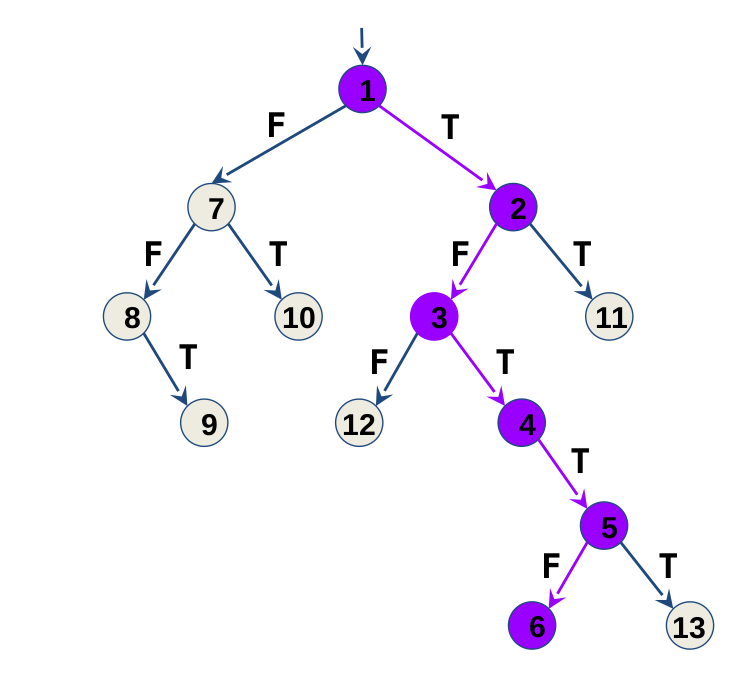
\includegraphics[scale=0.2]{tree.png}
\end{minipage}
\end{frame}

\begin{frame}[fragile]{Example}
\begin{minipage}{0.49\textwidth}
\begin{lstlisting}[language=C++]
void test(int x, int y) {
   if (2*y == x) {
      if (x <= y+10) {
         printf("OK");
      } else {
         printf("not OK");
         assert false;
      }
   } else {
      print("OK");
   }
}
\end{lstlisting}
\end{minipage}
\end{frame}

\begin{frame}[fragile]{Existed approach}
\begin{minipage}{0.49\textwidth}
\begin{lstlisting}[language=C++]
 void test(int x) {
     if (x == 94389) {
         assert false;
     }
 }
\end{lstlisting}
\end{minipage}
\begin{minipage}{0.49\textwidth}
\begin{itemize}
\item Random testion
\item The probability to detect error is very low
\end{itemize}
\end{minipage}
\end{frame}

\begin{frame}[fragile]{Symbolic execution}
\begin{minipage}{0.49\textwidth}
\begin{lstlisting}[language=C++]
void foo(int x, int y) {
    int t = 0;
    if (x > y) {
        t = x;
    } else {
        t = y;
    }
    if (t < x) {
        assert false;
    }
}
\end{lstlisting}
\end{minipage}
\hfill
\begin{minipage}{0.49\textwidth}
\begin{center}
\begin{tabular}{ | l | l | l | }
\hline
$X$ & $Y$ & $T$ \\
\hline
$x$ & $y$ & 0 \\
\hline
\end{tabular}
\end{center}
\end{minipage}
\end{frame}

\begin{frame}[fragile]{Symbolic execution}
\begin{minipage}{0.49\textwidth}
\begin{lstlisting}[language=C++]
void foo(int x, int y) {
    int t = 0;
    if (x > y) {
        t = x;
    } else {
        t = y;
    }
    if (t < x) {
        assert false;
    }
}
\end{lstlisting}
\end{minipage}
\hfill
\begin{minipage}{0.49\textwidth}
\begin{center}
\begin{tabular}{ | l | l | l | }
\hline
$X$ & $Y$ & $T$ \\
\hline
$x$ & $y$ & $t_0$ \\
\hline
\end{tabular}
\begin{equation*}
t_0 =
    \begin{cases}
    $x$ &\text{$x > y$}\\
    $y$ &\text{$x \le y$}
    \end{cases}
\end{equation*}
\end{center}
\end{minipage}
\end{frame}

\begin{frame}[fragile]{Symbolic execution}
\begin{minipage}{0.49\textwidth}
\begin{lstlisting}[language=C++]
void foo(int x, int y) {
    int t = 0;
    if (x > y) {
        t = x;
    } else {
        t = y;
    }
    if (t < x) {
        assert false;
    }
}
\end{lstlisting}
\end{minipage}
\hfill
\begin{minipage}{0.49\textwidth}
\begin{center}
\begin{tabular}{ | l | l | l | }
\hline
$X$ & $Y$ & $T$ \\
\hline
$x$ & $y$ & $t_0$ \\
\hline
\end{tabular}
\begin{equation*}
t_0 =
    \begin{cases}
    $x$ &\text{$x > y$}\\
    $y$ &\text{$x \le y$}
    \end{cases}
\end{equation*}
$t_0 < x?$
\end{center}
\end{minipage}
\end{frame}

\begin{frame}[fragile]{Symbolic execution}
\begin{minipage}{0.49\textwidth}
\begin{lstlisting}[language=C++]
void foo(int x, int y) {
    int t = 0;
    if (x > y) {
        t = x;
    } else {
        t = y;
    }
    if (t < x) {
        assert false;
    }
}
\end{lstlisting}
\end{minipage}
\hfill
\begin{minipage}{0.49\textwidth}
\begin{center}
\begin{tabular}{ | l | l | l | }
\hline
$X$ & $Y$ & $T$ \\
\hline
$x$ & $y$ & $t_0$ \\
\hline
\end{tabular}
\begin{equation*}
t_0 =
    \begin{cases}
    $x$ &\text{$x > y$}\\
    $y$ &\text{$x \le y$}
    \end{cases}
\end{equation*}
$\left\{
\begin{array}{l}
x > y \implies t_0 = x \implies t_0 \ge x \\
x \le y \implies t_0 = y \implies t_0 \ge x \\
\end{array}
\right.$
\end{center}
\end{minipage}
\end{frame}

\begin{frame}[fragile]{Symbolic execution}
\begin{minipage}{0.49\textwidth}
\begin{lstlisting}[language=C++]
void foo(int x, int y) {
    int t = 0;
    if (x > y) {
        t = x - 1;
    } else {
        t = y;
    }
    if (t < x) {
        assert false;
    }
}
\end{lstlisting}
\end{minipage}
\hfill
\begin{minipage}{0.49\textwidth}
\begin{center}
\begin{tabular}{ | l | l | l | }
\hline
$X$ & $Y$ & $T$ \\
\hline
$x$ & $y$ & $t_0$ \\
\hline
\end{tabular}
\end{center}
\end{minipage}
\end{frame}

\begin{frame}[fragile]{Symbolic execution}
\begin{minipage}{0.49\textwidth}
\begin{lstlisting}[language=C++]
void foo(int x, int y) {
    int t = 0;
    if (x > y) {
        t = x - 1;
    } else {
        t = y;
    }
    if (t < x) {
        assert false;
    }
}
\end{lstlisting}
\end{minipage}
\hfill
\begin{minipage}{0.49\textwidth}
\begin{center}
\begin{tabular}{ | l | l | l | }
\hline
$X$ & $Y$ & $T$ \\
\hline
$x$ & $y$ & $t_0$ \\
\hline
\end{tabular}
\begin{equation*}
t_0 =
    \begin{cases}
    $x - 1$ &\text{$x > y$}\\
    $y$ &\text{$x \le y$}
    \end{cases}
\end{equation*}
\end{center}
\end{minipage}
\end{frame}

\begin{frame}[fragile]{Symbolic execution}
\begin{minipage}{0.49\textwidth}
\begin{lstlisting}[language=C++]
void foo(int x, int y) {
    int t = 0;
    //if (x > y) {
        t = x - 1;
    //} else {
    //    t = y;
    //}
    //if (t < x) {
        assert false;
    //}
}
\end{lstlisting}
\end{minipage}
\hfill
\begin{minipage}{0.49\textwidth}
\begin{center}
\begin{tabular}{ | l | l | l | }
\hline
$X$ & $Y$ & $T$ \\
\hline
$x$ & $y$ & $t_0$ \\
\hline
\end{tabular}
\begin{equation*}
t_0 =
    \begin{cases}
    $x - 1$ &\text{$x > y$}\\
    $y$ &\text{$x \le y$}
    \end{cases}
\end{equation*}
$\left\{
\begin{array}{l}
x > y \implies t_0 = x - 1 \implies t_0 < x \\
x \le y \implies t_0 = y \implies t_0 \ge x \\
\end{array}
\right.$
$x > y$ - solution
\end{center}
\end{minipage}
\end{frame}

\begin{frame}[fragile]{Symbolic execution}
\begin{minipage}{0.49\textwidth}
\begin{lstlisting}[language=C++]
void testme(int x) {
   if (pow(2,x) % c == 17) {
      printf("not OK");
      assert false;
   } else
      printf("OK");
}
\end{lstlisting}
\end{minipage}
\end{frame}


\begin{frame}[fragile]{Concolic execution}
Concolic execution (or dynamic symbolic execution):
\begin{itemize}
\item Start with random input data
\item Track the conrete and symbolic variables
\end{itemize}
\end{frame}

\begin{frame}[fragile]{Concolic execution}
\begin{minipage}{0.49\textwidth}
\begin{lstlisting}[language=C++,escapechar=@]
void foo(int x, int y) {
    int t = 0;
    if (x > y) {
        t = x;
    } else {
        t = y;
    }
    if (t < x) {
        assert false;
    }
}
\end{lstlisting}
\end{minipage}
\hfill
\begin{minipage}{0.49\textwidth}
\begin{center}
\begin{tabular}{ | l | l | l | }
\hline
$X$ & $Y$ & $T$ \\
\hline
$x$ & $y$ & $t_0$ \\
\hline
\end{tabular}
\begin{equation*}
t_0 =
    \begin{cases}
    $x$ &\text{$x > y$}\\
    $y$ &\text{$x \le y$}
    \end{cases}
\end{equation*}
\end{center}
\end{minipage}
\end{frame}

\begin{frame}[fragile]{Concolic execution}
\begin{minipage}{0.49\textwidth}
\begin{lstlisting}[language=C++,escapechar=@]
void foo(int x, int y) {
    @\textbf{int t = 0;}@
    if (x > y) {
        t = x;
    } else {
        t = y;
    }
    if (t < x) {
        assert false;
    }
}
\end{lstlisting}
\end{minipage}
\hfill
\begin{minipage}{0.49\textwidth}
\begin{center}
\begin{tabular}{ | l | l | l | }
\hline
$X$ & $Y$ & $T$ \\
\hline
$(0, x)$ & $(0, y)$ & $(0, 0)$ \\
\hline
\end{tabular}
\end{center}
\end{minipage}
\end{frame}

\begin{frame}[fragile]{Concolic execution}
\begin{minipage}{0.49\textwidth}
\begin{lstlisting}[language=C++,escapechar=@]
void foo(int x, int y) {
    @\textbf{int t = 0;}@
    @\textbf{if (x > y) \{}@
        t = x;
    } else {
        t = y;
    }
    if (t < x) {
        assert false;
    }
}
\end{lstlisting}
\end{minipage}
\hfill
\begin{minipage}{0.49\textwidth}
\begin{center}
\begin{tabular}{ | l | l | l | }
\hline
$X$ & $Y$ & $T$ \\
\hline
$(0, x)$ & $(0, y)$ & $(0, 0)$ \\
\hline
\end{tabular}
\end{center}
\end{minipage}
\end{frame}

\begin{frame}[fragile]{Concolic execution}
\begin{minipage}{0.49\textwidth}
\begin{lstlisting}[language=C++,escapechar=@]
void foo(int x, int y) {
    @\textbf{int t = 0;}@
    @\textbf{if (x > y) \{}@
        t = x;
    } else {
        t = y;
    }
    if (t < x) {
        assert false;
    }
}
\end{lstlisting}
\end{minipage}
\hfill
\begin{minipage}{0.49\textwidth}
\begin{center}
\begin{tabular}{ | l | l | l | }
\hline
$X$ & $Y$ & $T$ \\
\hline
$(0, x)$ & $(0, y)$ & $(0, 0)$ \\
\hline
\end{tabular}
$\left\{
\begin{array}{l}
F1 = not (x > y)
\end{array}
\right.$
\end{center}
\end{minipage}
\end{frame}

\begin{frame}[fragile]{Concolic execution}
\begin{minipage}{0.49\textwidth}
\begin{lstlisting}[language=C++,escapechar=@]
void foo(int x, int y) {
    @\textbf{int t = 0;}@
    @\textbf{if (x > y) \{}@
        t = x;
    } else {
        t = y;
    }
    if (t < x) {
        assert false;
    }
}
\end{lstlisting}
\end{minipage}
\hfill
\begin{minipage}{0.49\textwidth}
\begin{center}
\begin{tabular}{ | l | l | l | }
\hline
$X$ & $Y$ & $T$ \\
\hline
$(0, x)$ & $(0, y)$ & $(0, 0)$ \\
\hline
\end{tabular}
$\left\{
\begin{array}{l}
F1 = not (x > y)
\end{array}
\right.$
$SMT\_Solver($not $F1) \to (x = 1, y = 0)$
\end{center}
\end{minipage}
\end{frame}

\begin{frame}[fragile]{Concolic execution}
\begin{minipage}{0.49\textwidth}
\begin{lstlisting}[language=C++,escapechar=@]
void foo(int x, int y) {
    @\textbf{int t = 0;}@
    @\textbf{if (x > y) \{}@
        t = x;
    } else {
        t = y;
    }
    if (t < x) {
        assert false;
    }
}
\end{lstlisting}
\end{minipage}
\hfill
\begin{minipage}{0.49\textwidth}
\begin{center}
\begin{tabular}{ | l | l | l | }
\hline
$X$ & $Y$ & $T$ \\
\hline
$(0, x)$ & $(0, y)$ & $(0, 0)$ \\
\hline
\end{tabular}
$\left\{
\begin{array}{l}
F1 = not (x > y)
\end{array}
\right.$
$SMT\_Solver($not $F1) \to (x = 1, y = 0)$
$queue = \{(x = 1, y = 0)\}$
\end{center}
\end{minipage}
\end{frame}

\begin{frame}[fragile]{Concolic execution}
\begin{minipage}{0.49\textwidth}
\begin{lstlisting}[language=C++,escapechar=@]
void foo(int x, int y) {
    @\textbf{int t = 0;}@
    @\textbf{if (x > y) \{}@
        t = x;
    @\textbf{\} else \{}@
        t = y;
    }
    if (t < x) {
        assert false;
    }
}
\end{lstlisting}
\end{minipage}
\hfill
\begin{minipage}{0.49\textwidth}
\begin{center}
\begin{tabular}{ | l | l | l | }
\hline
$X$ & $Y$ & $T$ \\
\hline
$(0, x)$ & $(0, y)$ & $(0, 0)$ \\
\hline
\end{tabular}
$\left\{
\begin{array}{l}
F1 = not (x > y)
\end{array}
\right.$
$queue = \{(x = 1, y = 0)\}$
\end{center}
\end{minipage}
\end{frame}

\begin{frame}[fragile]{Concolic execution}
\begin{minipage}{0.49\textwidth}
\begin{lstlisting}[language=C++,escapechar=@]
void foo(int x, int y) {
    @\textbf{int t = 0;}@
    @\textbf{if (x > y) \{}@
        t = x;
    @\textbf{\} else \{}@
        @\textbf{t = y;}@
    }
    if (t < x) {
        assert false;
    }
}
\end{lstlisting}
\end{minipage}
\hfill
\begin{minipage}{0.49\textwidth}
\begin{center}
\begin{tabular}{ | l | l | l | }
\hline
$X$ & $Y$ & $T$ \\
\hline
$(0, x)$ & $(0, y)$ & $(0, y)$ \\
\hline
\end{tabular}
$\left\{
\begin{array}{l}
F1 = not (x > y)
\end{array}
\right.$
$queue = \{(x = 1, y = 0)\}$
\end{center}
\end{minipage}
\end{frame}

\begin{frame}[fragile]{Concolic execution}
\begin{minipage}{0.49\textwidth}
\begin{lstlisting}[language=C++,escapechar=@]
void foo(int x, int y) {
    @\textbf{int t = 0;}@
    @\textbf{if (x > y) \{}@
        t = x;
    @\textbf{\} else \{}@
        @\textbf{t = y;}@
    @\textbf{\}}@
    if (t < x) {
        assert false;
    }
}
\end{lstlisting}
\end{minipage}
\hfill
\begin{minipage}{0.49\textwidth}
\begin{center}
\begin{tabular}{ | l | l | l | }
\hline
$X$ & $Y$ & $T$ \\
\hline
$(0, x)$ & $(0, y)$ & $(0, y)$ \\
\hline
\end{tabular}
$\left\{
\begin{array}{l}
F1 = not (x > y)
\end{array}
\right.$
$queue = \{(x = 1, y = 0)\}$
\end{center}
\end{minipage}
\end{frame}

\begin{frame}[fragile]{Concolic execution}
\begin{minipage}{0.49\textwidth}
\begin{lstlisting}[language=C++,escapechar=@]
void foo(int x, int y) {
    @\textbf{int t = 0;}@
    @\textbf{if (x > y) \{}@
        t = x;
    @\textbf{\} else \{}@
        @\textbf{t = y;}@
    @\textbf{\}}@
    @\textbf{if (t < x) \{}@
        assert false;
    }
}
\end{lstlisting}
\end{minipage}
\hfill
\begin{minipage}{0.49\textwidth}
\begin{center}
\begin{tabular}{ | l | l | l | }
\hline
$X$ & $Y$ & $T$ \\
\hline
$(0, x)$ & $(0, y)$ & $(0, y)$ \\
\hline
\end{tabular}
$\left\{
\begin{array}{l}
F1 = not (x > y)
\end{array}
\right.$
$queue = \{(x = 1, y = 0)\}$
\end{center}
\end{minipage}
\end{frame}

\begin{frame}[fragile]{Concolic execution}
\begin{minipage}{0.49\textwidth}
\begin{lstlisting}[language=C++,escapechar=@]
void foo(int x, int y) {
    @\textbf{int t = 0;}@
    @\textbf{if (x > y) \{}@
        t = x;
    @\textbf{\} else \{}@
        @\textbf{t = y;}@
    @\textbf{\}}@
    @\textbf{if (t < x) \{}@
        assert false;
    }
}
\end{lstlisting}
\end{minipage}
\hfill
\begin{minipage}{0.49\textwidth}
\begin{center}
\begin{tabular}{ | l | l | l | }
\hline
$X$ & $Y$ & $T$ \\
\hline
$(0, x)$ & $(0, y)$ & $(0, y)$ \\
\hline
\end{tabular}
$\left\{
\begin{array}{l}
F1 = not (x > y) \\
F2 = not (y < x)
\end{array}
\right.$
$queue = \{(x = 1, y = 0)\}$
\end{center}
\end{minipage}
\end{frame}

\begin{frame}[fragile]{Concolic execution}
\begin{minipage}{0.49\textwidth}
\begin{lstlisting}[language=C++,escapechar=@]
void foo(int x, int y) {
    @\textbf{int t = 0;}@
    @\textbf{if (x > y) \{}@
        t = x;
    @\textbf{\} else \{}@
        @\textbf{t = y;}@
    @\textbf{\}}@
    @\textbf{if (t < x) \{}@
        assert false;
    }
}
\end{lstlisting}
\end{minipage}
\hfill
\begin{minipage}{0.49\textwidth}
\begin{center}
\begin{tabular}{ | l | l | l | }
\hline
$X$ & $Y$ & $T$ \\
\hline
$(0, x)$ & $(0, y)$ & $(0, y)$ \\
\hline
\end{tabular}
$\left\{
\begin{array}{l}
F1 = not (x > y) \\
F2 = not (y < x)
\end{array}
\right.$
$SMT\_Solver(F1$ and not $F2) \to UNSAT$
$queue = \{(x = 1, y = 0)\}$
\end{center}
\end{minipage}
\end{frame}

\begin{frame}[fragile]{Concolic execution}
\begin{minipage}{0.49\textwidth}
\begin{lstlisting}[language=C++,escapechar=@]
void foo(int x, int y) {
    @\textbf{int t = 0;}@
    @\textbf{if (x > y) \{}@
        t = x;
    @\textbf{\} else \{}@
        @\textbf{t = y;}@
    @\textbf{\}}@
    @\textbf{if (t < x) \{}@
        assert false;
    @\textbf{\}}@
}
\end{lstlisting}
\end{minipage}
\hfill
\begin{minipage}{0.49\textwidth}
\begin{center}
\begin{tabular}{ | l | l | l | }
\hline
$X$ & $Y$ & $T$ \\
\hline
$(0, x)$ & $(0, y)$ & $(0, y)$ \\
\hline
\end{tabular}
$\left\{
\begin{array}{l}
F1 = not (x > y) \\
F2 = not (y < x)
\end{array}
\right.$
$queue = \{(x = 1, y = 0)\}$
\end{center}
\end{minipage}
\end{frame}

\begin{frame}[fragile]{Concolic execution}
\begin{minipage}{0.49\textwidth}
\begin{lstlisting}[language=C++,escapechar=@]
void foo(int x, int y) {
    int t = 0;
    if (x > y) {
        t = x;
    } else {
        t = y;
    }
    if (t < x) {
        assert false;
    }
}
\end{lstlisting}
\end{minipage}
\hfill
\begin{minipage}{0.49\textwidth}
\begin{center}
\begin{tabular}{ | l | l | l | }
\hline
$X$ & $Y$ & $T$ \\
\hline
$(1, x)$ & $(0, y)$ & $(0, 0)$ \\
\hline
\end{tabular}
$queue = \{\}$
\end{center}
\end{minipage}
\end{frame}

\begin{frame}[fragile]{Example}
\begin{minipage}{0.49\textwidth}
\begin{lstlisting}[language=C++]
int test(int x) {
   int[] A = { 5, 7, 9 };
   int i = 0;
   while (i < 3) {
      if (A[i] == x) {
          break;
      }
      i++;
   }
   return i;
}
\end{lstlisting}
\end{minipage}
\begin{minipage}{0.49\textwidth}
\end{minipage}
\end{frame}

\begin{frame}[fragile]{Exampl}
\begin{minipage}{0.40\textwidth}
\begin{lstlisting}[language=C++]
int foo(int v) {
   return secure_hash(v);
}

void test(int x, int y) {
   if (x != y)
      if (foo(x) == foo(y))
         assert;
}
\end{lstlisting}
\end{minipage}
\hfill
\begin{minipage}{0.40\textwidth}
\end{minipage}
\end{frame}

\begin{frame}{Consolic Execution}
\begin{itemize}
\item Could never stop execution
\item Sound
\item Not complete
\end{itemize}
\end{frame}

\begin{frame}[fragile]{Implementation}
\begin{lstlisting}[language=python,escapechar=@]
a = b + c
\end{lstlisting}
\end{frame}

\begin{frame}[fragile]{Implementation}
\begin{lstlisting}[language=python,escapechar=@]
class concolic_int(int):
def __new__(cls, val, sym):
    self =
     super(concolic_int, cls).__new__(cls, val)
    self.__val = val
    self.__sym = sym
    return self
def __add__(self, other):
    if isinstance(other, concolic_int):
        value = self.__val + other.__val
        symbolic = self.__sym + "+" + other.__sym
    else:
        value = self.__val + other
        symbolic = self.__sym + "+" + str(other)
    return concolic_int(value, symbolic)
\end{lstlisting}
\end{frame}

\begin{frame}[fragile]{Implementation}
How could one change int on concolic\_int?
\end{frame}

\begin{frame}[fragile]{Implementation}
\begin{lstlisting}[language=python,escapechar=@]
a = b + c
\end{lstlisting}
\end{frame}

\begin{frame}[fragile]{Implementation}
\begin{lstlisting}[language=python,escapechar=@]
a = plus(b, c)
\end{lstlisting}
\end{frame}

\begin{frame}[fragile]{Implementation}
\begin{lstlisting}[language=python,escapechar=@]
function plus(x, y) {
    if (x isinstanceof Concolic) {
        if (y isinstanceof Concolic) {
            return new Concolic(
                x._val + y._val,
                x._sym + "+" + y._sym
            );
        } else {
            return new Concolic(
                x._val + y,
                x._sym + "+" + y.toString()
            );
        }
    } else {
        ....
    }
}
\end{lstlisting}
\end{frame}

\begin{frame}[fragile]{Implementation}
How to ecode the pathes?
\end{frame}

\begin{frame}{Examples}
\begin{itemize}
\item KLEE: LLVM (C family of languages)
\item PEX: .NET Framework
\item CUTE: C
\item jCUTE: Java
\item Jalangi: Javascript
\item Jalangi2 + ExpoSE: Javascript
\item SAGE and S2E: binaries (x86, ARM, ...)
\end{itemize}
\end{frame}

\begin{frame}{Links}
\begin{itemize}
\item https://www.youtube.com/watch?v=yRVZPvHYHzw - MIT lecture
\item Symbolic Execution and Program Testing. James C. King
\item SAGE: Whitebox Fuzzing for Security Testing. Patrice Godefroid, Michael Y. Levin, and David A. Molnar
\item Jalangi: A Selective Record-Replay and Dynamic Analysis Framework for JavaScript. Koushik Sen, Swaroop Kalasapur, Tasneem Brutch, Simon Gibbs
\item Sound Regular Expression Semantics for Dynamic Symbolic Execution of JavaScript. Blake Loring, Duncan Mitchell, Johannes Kinder
\end{itemize}
\end{frame}

\begin{frame}
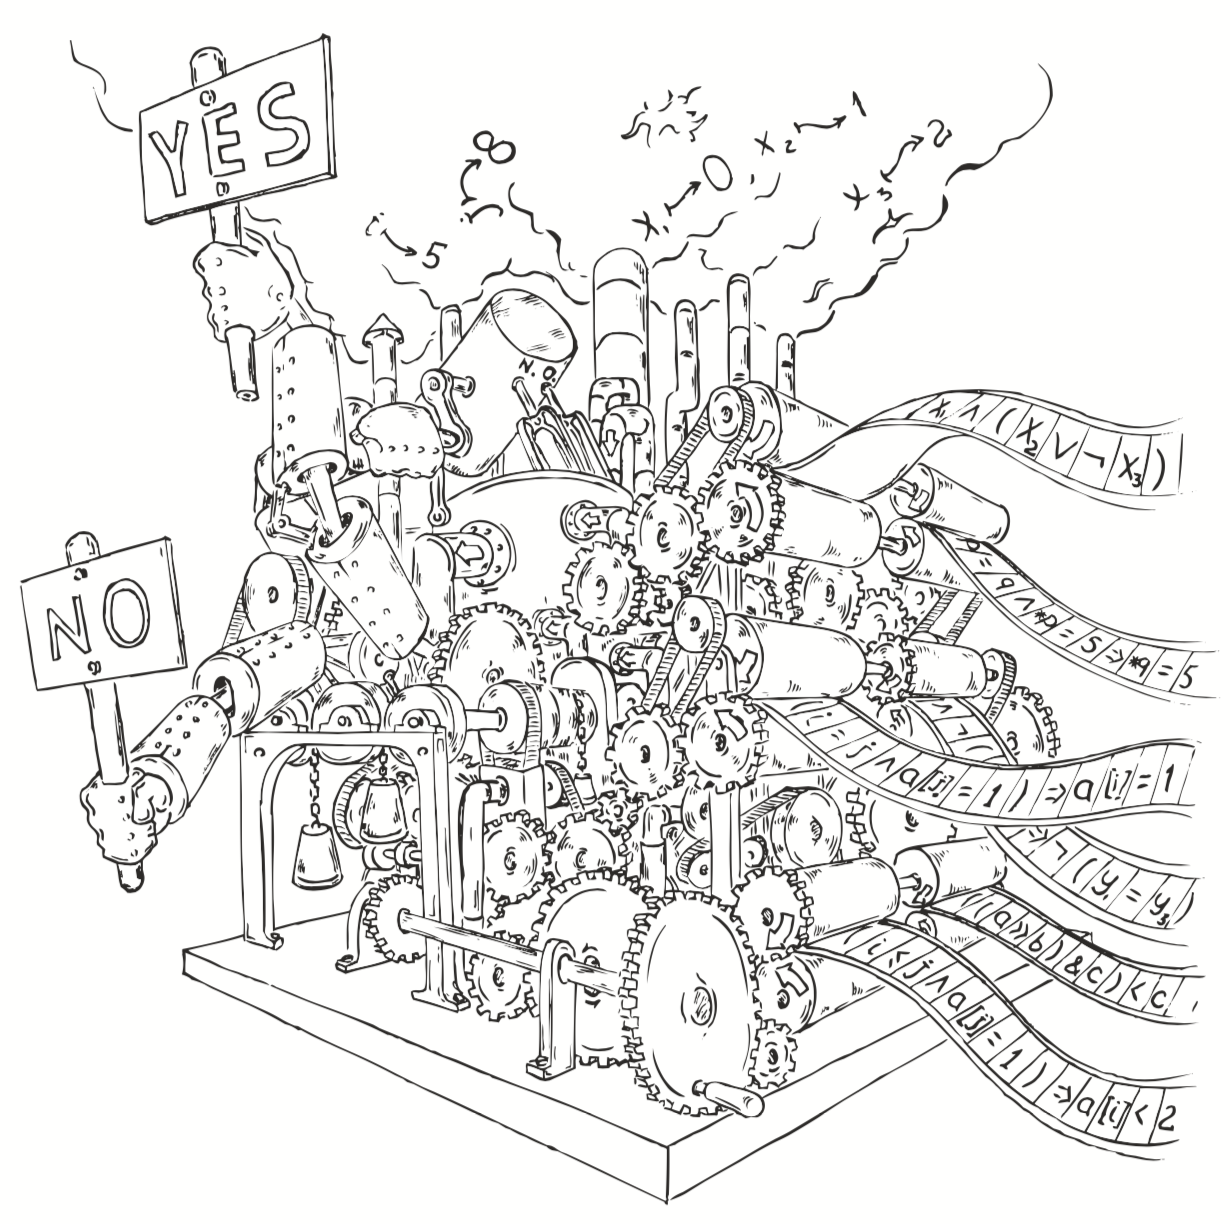
\includegraphics[scale=0.5]{../decision-procedure.png}
\end{frame}

\end{document}
